\chapter{Gerador}
\label{cap:p1}


O \textit{generator} é um programa que é capaz de receber e interpretar pedidos do utilizador para desenho de figuras e gerar um ficheiro '.3d' com os pontos correspondentes à figura pedida. A lista de pontos está ordenada de forma a formarem triângulos que juntos desenham a figura desejada. 

Nesta primeira etapa, o objetivo implementar o suporte à criação de um plano, uma caixa, um cone e uma esfera. 


\section{Funcionamento}

Nesta primeira fase o \textit{generator} é capaz de criar diversas primitivas gráficas
diferentes, entre as quais: \textit{plane} (plano), \textit{box} (paralelepípedo), \textit{sphere} (esfera), \textit{cone}. Para cada uma das primitivas geométricas é possível gerar o ficheiro correspondente através dos comandos:

\begin{itemize}
	\item PLANE: generator plano/plane <comprimento largura> <ficheiro>, onde a largura e comprimento são opcionais 
	
	\item BOX: generator box/caixa <sizeX sixeY sizeZ divisões> <ficheiro>, onde existe a possibilidade de as divisões serem opcionais
	
	\item SPHERE: generator sphere/esfera <raio fatias camadas> <ficheiro>
	
	\item CONE: generator cone <raio altura fatias camadas> <ficheiro>
	
\end{itemize}


Para a criação das formas geométricas é preciso obedecer a algumas restrições
com a passagem de argumentos, o primeiro parâmetro a ser passado deverá
ser o nome da figura a desenhar, o último será o nome do ficheiro onde será
guardada a lista de pontos, sendo a extensão “.3d” adicionada automaticamente
pelo generator. Sendo isto obedecido, o número de argumentos entre
o nome da figura e o nome do ficheiro varia consoante o tipo de figura a ser
criada, mas esses argumentos deverão ser numerais.


\section{Algoritmo de Geração de Pontos}


\section{Programa principal}

O pseudo-código do programa principal é o seguinte:


\begin{Verbatim}
int main(int argc, char** argv) {
Declara figura onde vao ser guardados os pontos
figuraCriada = false;

if (figura pedida == plano) {
Lê e interpreta parametros
Chama funçao da figura para desenhar os pontos 
de um plano
Grava pontos em ficheiro
figuraCriada = true;
}

if (figura pedida == caixa) {
Lê e interpreta parametros
Chama funçao da figura para desenhar os pontos
de uma caixa
Grava pontos em ficheiro
figuraCriada = true;
}

if (figura pedida == cone) {
Lê e interpreta parametros
Chama funçao da figura para desenhar os pontos 
de um cone
Grava pontos em ficheiro
figuraCriada = true;
}

if (figura pedida == esfera) {
Lê e interpreta parametros
Chama funçao da figura para desenhar os pontos
de uma esfera
Grava pontos em ficheiro
figuraCriada = true;
}


if (!figuraCriada) {
if (o programa for corrido sem argumentos) {
Informar utilizador que programa 
foi corrido sem argumentos
}
else {
Informar utilizador que nao foi possivel
criar a figura
}
Mostra mensagem de ajuda com sintaxe dos comandos
}

return 0;
}
\end{Verbatim}

\section{Primitivas}

Nesta secção apresentam-se os comandos correspondentes aos pedidos de figuras que o utilizador pode fazer e é explicada a sua implementação.

\subsection{Gerar Planos}
\label{p1:planos}

Para gerar um plano, o utilizador deve efetuar o comando com a seguinte sintaxe:

\begin{Verbatim}
Gerador plane comprimento largura ficheiro
\end{Verbatim}

O resultado deste comando é a criação de um plano em XZ centrado no ponto (0,0,0) com o comprimento e largura indicados.

\subsubsection{Plano em XZ (Y=constante)}

Um plano é formado por 2 triângulos. Com a informação de 4 pontos é possível desenhar esses triângulos. A figura \ref{p1:fig:p1_planoY} representa um plano em XZ. De notar que é possível considerar dois triângulos: o triângulo formado por [ABC] e o triângulo formado por [CDA]

\begin{figure}[<+htpb+>]
	\centering
	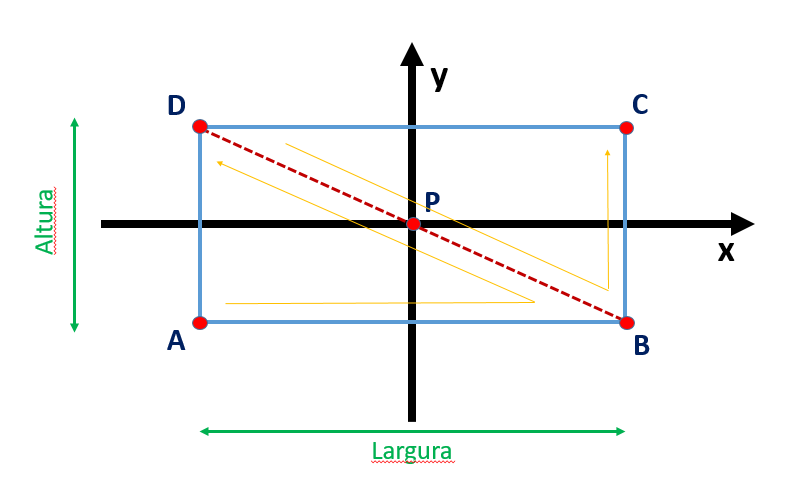
\includegraphics[scale=0.5]{imagens/p3_planoY.png}
	\caption{Plano em XZ centrado na origem}
	\label{p1:fig:p1_planoY}
\end{figure}

Estando o plano centrado na origem, e sabendo o comprimento e largura do plano, conclui-se que as coordenadas dos pontos da figura \ref{p1:fig:p1_planoY} são as seguintes:

\begin{Verbatim}
A(-comprimento/2, 0, -largura/2)
B(-comprimento/2, 0, largura/2)
C(comprimento/2, 0, largura/2)
P(0, 0, 0)
\end{Verbatim}

É também fácil exprimir as coordenadas de um plano não necessariamente centrado na origem, em função do seu centro P:

\begin{Verbatim}
A(-comprimento/2 + px, 0 + py, -largura/2 + pz)
B(-comprimento/2 + px, 0 + py, largura/2 + pz)
C(comprimento/2 + px, 0 + py, largura/2 + pz)
P(px, py, pz)
\end{Verbatim}

A ordem pela qual se adiciona os pontos à figura determina para que lado ela fica virada. Se quisermos que o plano fique virado para o sentido positivo do eixo dos Y, deve-se colocar os pontos pela seguinte ordem: A-B-C (1º triângulo), seguido de C-D-A (2º triângulo). Se quisermos que o plano fique virado para o sentido negativo do eixo dos Y, deve-se colocar os pontos pela seguinte ordem: A-D-C (1º triângulo), seguido de C-B-A (2º triângulo).

A função responsável por implementar este algoritmo é a função \textit{criaPlanoEmY()}, cujo pseudo-código se apresenta de seguida:

\begin{Verbatim}
Figura& criaPlanoEmY(Ponto3D centroPlano, float comprimento, 
float largura, int orientacao) {

Calcula coordendas dos pontos A,B,C e D

if (orientacao == 1) {
Coloca pontos pela ordem A-B-C-C-D-A
}
else {
Coloca pontos pela ordem A-D-C-C-B-A
}

return *this;
}
\end{Verbatim}

De notar que esta função além do comprimento e largura, recebe ainda o centro do plano e a orientação do mesmo.

\begin{figure}[<+htpb+>]
	\centering
	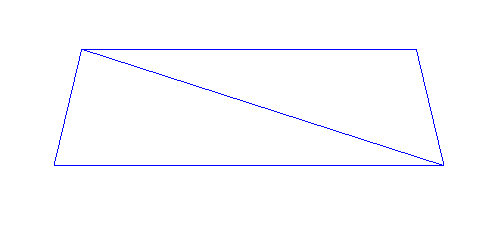
\includegraphics[scale=0.5]{imagens/p3_plano_4_2.png}
	\caption{Exemplo de plano em XZ gerado, com 4 de comprimento e 2 de largura}
	\label{p1:fig:p3_plano_4_2}
\end{figure}

\subsubsection{Plano em XY (Z=constante)}

Embora apenas fosse pedido que o gerador tivesse a capacidade de gerar um plano em XZ, considerou-se útil disponibilizar também uma primitiva para criar planos em XY.
Um plano é formado por 2 triângulos. Com a informação de 4 pontos é possível desenhar esses triângulos. A figura \ref{p1:fig:p3_planoZ} representa um plano em XY. De notar que é possível considerar dois triângulos: o triângulo formado por [ABC] e o triângulo formado por [CDA]

\begin{figure}[<+htpb+>]
	\centering
	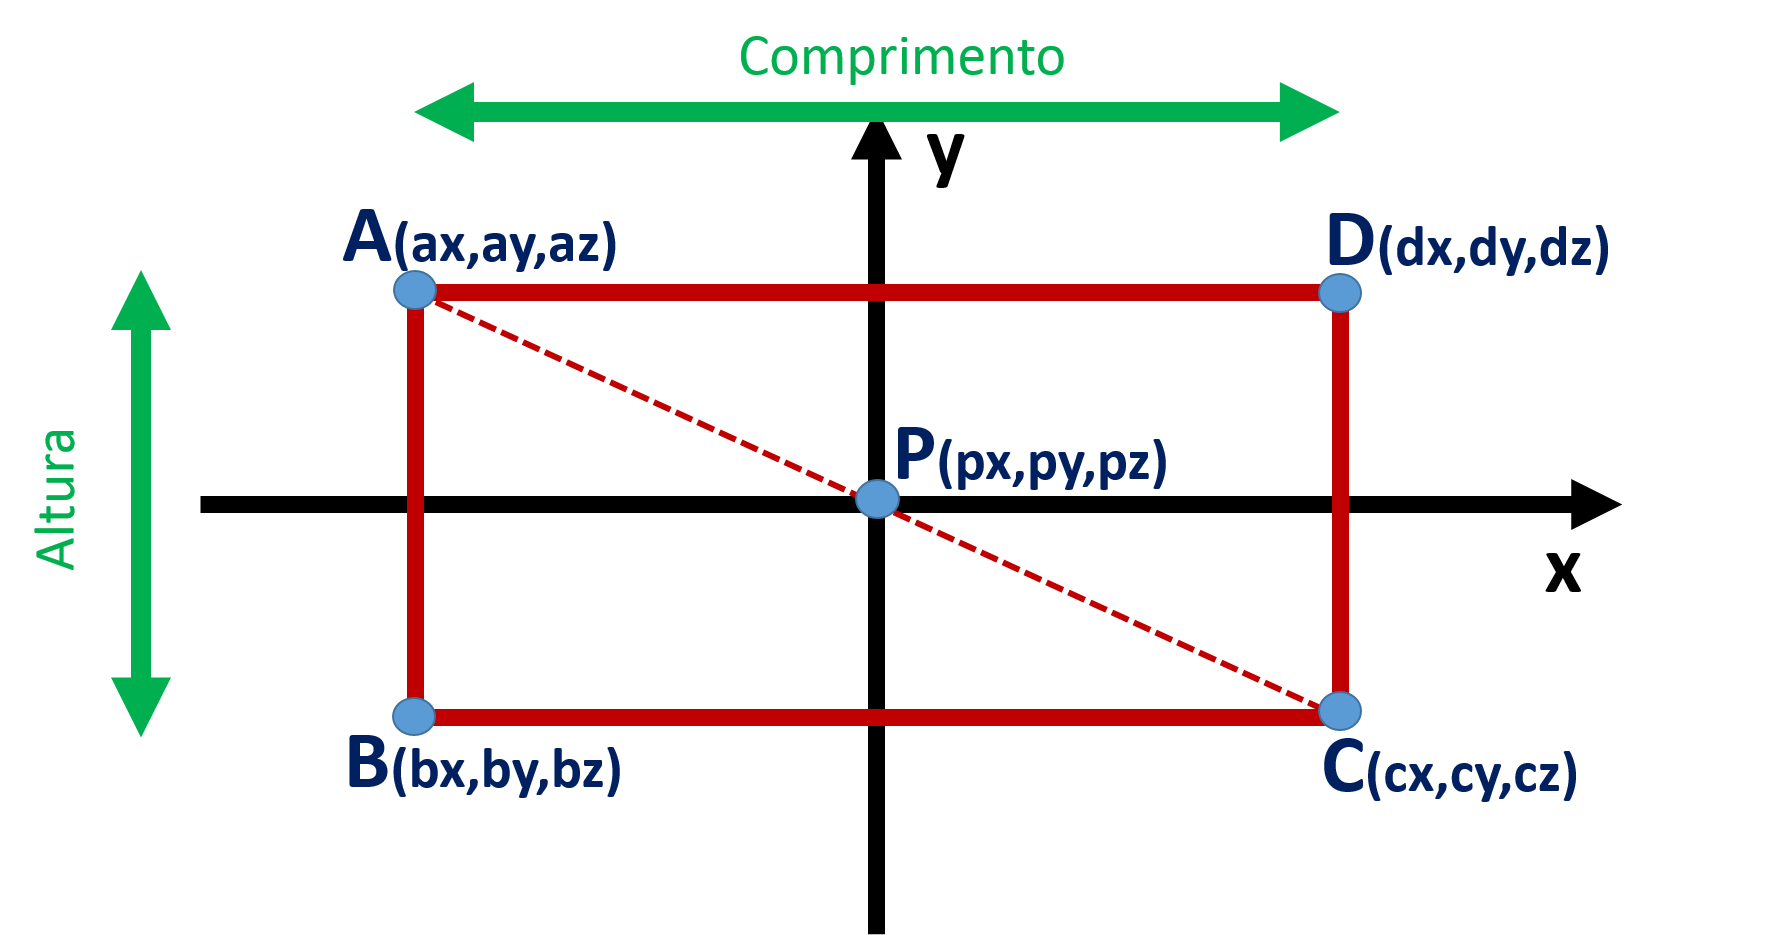
\includegraphics[scale=0.5]{imagens/p3_planoZ.png}
	\caption{Plano em XZ centrado na origem}
	\label{p1:fig:p3_planoZ}
\end{figure}

Estando o plano centrado na origem, e sabendo o comprimento e largura do plano, conclui-se que as coordenadas dos pontos da figura \ref{p1:fig:p3_planoZ} são as seguintes:

\begin{Verbatim}
A(-comprimento/2 , altura/2, 0)
B(-comprimento/2 , -altura/2, 0)
C(comprimento/2 , -altura/2, 0)
D(comprimento/2 , altura/2, 0)
P(0,0,0)
\end{Verbatim}

É também fácil exprimir as coordenadas de um plano não necessariamente centrado na origem, em função do seu centro P:

\begin{Verbatim}
A(-comprimento/2 + px, altura/2 + py, 0 + pz)
B(-comprimento/2 + px, -altura/2 + py, 0 + pz)
C(comprimento/2 + px, -altura/2 + py, 0 + pz)
D(comprimento/2 +px, altura/2 + py, 0 + pz)
P(px, py, pz)
\end{Verbatim}

A ordem pela qual se adiciona os pontos à figura determina para que lado ela fica virada. Se quisermos que o plano fique virado para o sentido positivo do eixo dos Y, deve-se colocar os pontos pela seguinte ordem: A-B-C (1º triângulo), seguido de C-D-A (2º triângulo). Se quisermos que o plano fique virado para o sentido negativo do eixo dos Y, deve-se colocar os pontos pela seguinte ordem: A-D-C (1º triângulo), seguido de C-B-A (2º triângulo).

A função responsável por implementar este algoritmo é a função \textit{criaPlanoEmZ()}, cujo pseudo-código se apresenta de seguida:

\begin{Verbatim}
Figura& criaPlanoEmZ(Ponto3D centroPlano, float comprimento, 
float altura, int orientacao) {

Calcula coordendas dos pontos A,B,C e D

if (orientacao == 1) {
Coloca pontos pela ordem A-B-C-C-D-A
}
else {
Coloca pontos pela ordem A-D-C-C-B-A
}

return *this;
}
\end{Verbatim}

De notar que esta função além do comprimento e altura, recebe ainda o centro do plano e a orientação do mesmo.

\subsubsection{Plano em YZ (X=constante)}

Embora apenas fosse pedido que o gerador tivesse a capacidade de gerar um plano em XZ, considerou-se útil disponibilizar também uma primitiva para criar planos em YZ.
Um plano é formado por 2 triângulos. Com a informação de 4 pontos é possível desenhar esses triângulos. A figura \ref{p1:fig:p3_planoX} representa um plano em YZ. De notar que é possível considerar dois triângulos: o triângulo formado por [ABC] e o triângulo formado por [CDA]

\begin{figure}[<+htpb+>]
	\centering
	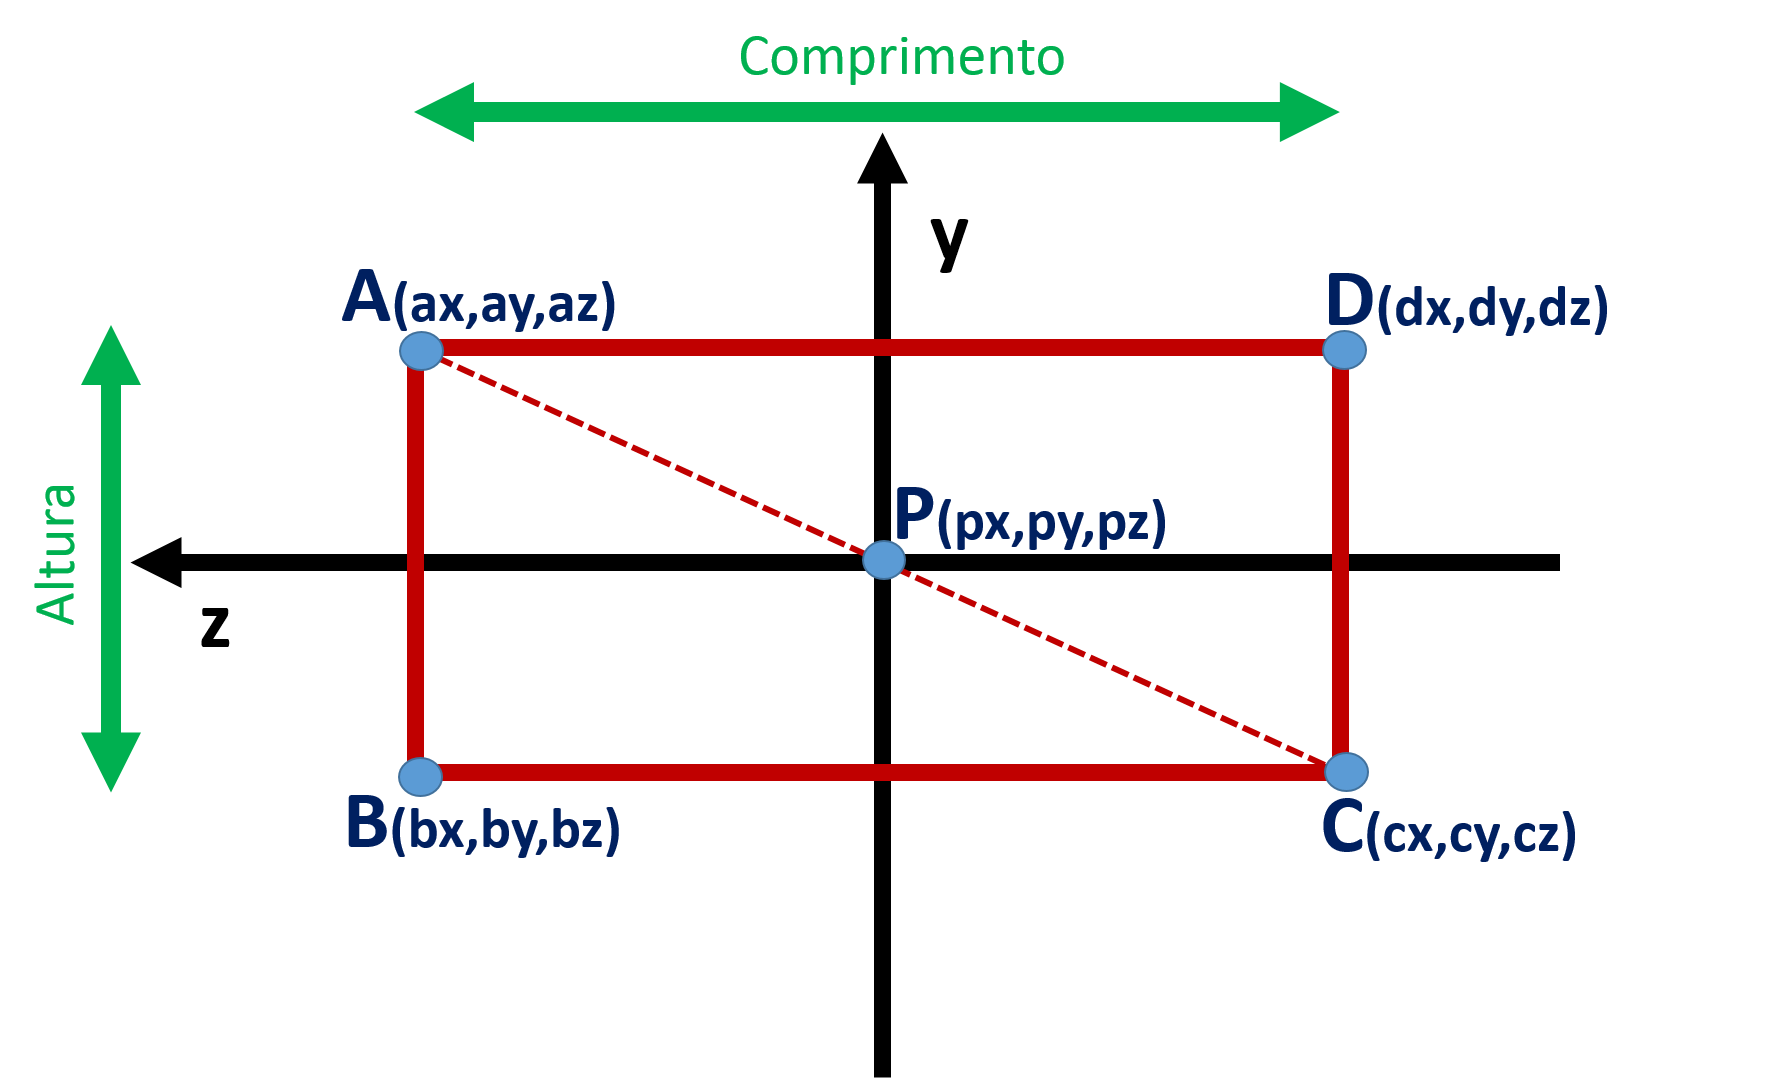
\includegraphics[scale=0.5]{imagens/p3_planoX.png}
	\caption{Plano em XZ centrado na origem}
	\label{p1:fig:p3_planoX}
\end{figure}

Estando o plano centrado na origem, e sabendo o comprimento e largura do plano, conclui-se que as coordenadas dos pontos da figura \ref{p1:fig:p3_planoX} são as seguintes:

\begin{Verbatim}
A(0, altura/2, comprimento/2)
B(0, -altura/2, comprimento/2)
C(0, -altura/2, -comprimento/2)
D(0, altura/2, -comprimento/2)
P(0,0,0)
\end{Verbatim}

É também fácil exprimir as coordenadas de um plano não necessariamente centrado na origem, em função do seu centro P:

\begin{Verbatim}
A(0 + px, altura/2 + py, comprimento/2 + pz)
B(0 + px, -altura/2 + py, comprimento/2 + pz)
C(0 + px, -altura/2 + py, -comprimento/2 + pz)
D(0 + px, altura/2 + py, -comprimento/2 + pz)
P(px, py, pz)
\end{Verbatim}

A ordem pela qual se adiciona os pontos à figura determina para que lado ela fica virada. Se quisermos que o plano fique virado para o sentido positivo do eixo dos Y, deve-se colocar os pontos pela seguinte ordem: A-B-C (1º triângulo), seguido de C-D-A (2º triângulo). Se quisermos que o plano fique virado para o sentido negativo do eixo dos Y, deve-se colocar os pontos pela seguinte ordem: A-D-C (1º triângulo), seguido de C-B-A (2º triângulo).

A função responsável por implementar este algoritmo é a função \textit{criaPlanoEmX()}, cujo pseudo-código se apresenta de seguida:

\begin{Verbatim}
Figura& criaPlanoEmX(Ponto3D centroPlano, float comprimento, 
float altura, int orientacao) {

Calcula coordendas dos pontos A,B,C e D

if (orientacao == 1) {
Coloca pontos pela ordem A-B-C-C-D-A
}
else {
Coloca pontos pela ordem A-D-C-C-B-A
}

return *this;
}
\end{Verbatim}

De notar que esta função além do comprimento e altura, recebe ainda o centro do plano e a orientação do mesmo.

\subsection{Gerar Caixa}

Para gerar uma caixa, o utilizador deve efetuar o comando com a seguinte sintaxe:

\begin{Verbatim}
Gerador caixa comprimento largura altura ficheiro
\end{Verbatim}

O resultado deste comando é a criação de uma caixa centrada no ponto (0,0,0) com o comprimento, largura e altura indicados.

Na secção \ref{p3:planos} foram apresentadas as primitivas que permitiam fazer planos. Nomeadamente viu-se que essas primitivas permitiam geral planos em XY, YZ e XZ dado um centro e uma orientação.

Uma caixa é apenas um conjunto de planos. Assim, para gerar a caixa o que se fez foi gerar os seus planos usando as primitivas da secção \ref{p3:planos}. No entanto, para usar tais primitivas é necessário indicar um centro do plano e uma orientação para o mesmo. É por isso necessário calcular esses parâmetros antes de usar as primitivas dos planos.

Considere-se a caixa com as faces visíveis identificadas pelas letras A, B e C, conforme mostra a figura \ref{p1:fig:p3_Caixa}

\begin{figure}[<+htpb+>]
	\centering
	\includegraphics[scale=0.5]{imagens/p3_Caixa.png}
	\caption{Esquema representativo da caixa}
	\label{p1:fig:p3_Caixa}
\end{figure}

Considere-se ainda que a face oposta a A é designada por A', a face oposta a B por B' e a face oposta a C por C'.
Interessa agora saber as coordenadas dos centros de cada uma destas faces. Considerando a caixa centrada na origem, temos o seguinte:

\begin{Verbatim}
Centro A  = (0,altura/2,0)          Orientação = 1
Centro A' = (0,-altura/2,0)         Orientação = 0
Centro B  = (0,0,largura/2)         Orientação = 1
Centro B' = (0,0,-largura/2)        Orientação = 0
Centro C  = (comprimento/2,0,0)     Orientação = 1
Centro C' = (-comprimento/2,0,0)    Orientação = 0
\end{Verbatim}

O valor da orientação toma o valor 1 se o plano estiver virado no sentido positivo do eixo sobre o qual esta colocado.

É fácil verificar que caso a caixa não esteja centrada na origem mas esteja centrada num ponto P(px, py, pz) as coordenadas dos centros das faces serão:

\begin{Verbatim}
Centro A  = (0 + px,altura/2 + py,0 + pz)          Orientação = 1
Centro A' = (0 + px,-altura/2 + py,0 + pz)         Orientação = 0
Centro B  = (0 + px,0 + py,largura/2 + pz)         Orientação = 1
Centro B' = (0 + px,0 + py,-largura/2 + pz)        Orientação = 0
Centro C  = (comprimento/2 + px,0 + py,0 + pz)     Orientação = 1
Centro C' = (-comprimento/2 + px,0 + py,0 + pz)    Orientação = 0
\end{Verbatim}

A função da classe \textit{Figura} responsável por gerar os pontos de uma caixa é a função \textit{criaCaixa()} cujo pseudo-código se apresenta a seguir:

\begin{Verbatim}
Figura& criaCaixa(Ponto3D centroCaixa, 
float dx, float dy, float dz) {

Calcula coordendas centro A
Cria plano com centro em A e orientacao = 1

Calcula coordendas centro A'
Cria plano com centro em A' e orientacao = 0

Calcula coordendas centro B
Cria plano com centro em B e orientacao = 1

Calcula coordendas centro B'
Cria plano com centro em B' e orientacao = 0

Calcula coordendas centro C
Cria plano com centro em C e orientacao = 1

Calcula coordendas centro C'
Cria plano com centro em C' e orientacao = 0

return *this;
}

\end{Verbatim}

\begin{figure}[<+htpb+>]
	\centering
	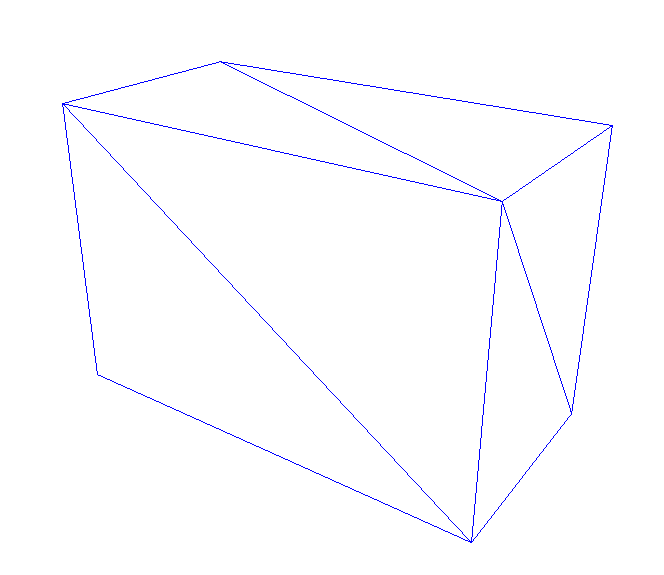
\includegraphics[scale=0.5]{imagens/p3_caixa_6_3_4.png}
	\caption{Exemplo de caixa gerada, com 6 de comprimento, 3 de largura e 4 de altura}
	\label{p1:fig:p3_caixa_6_3_4}
\end{figure}

\newpage
\subsection{Gerar Círculo}
\label{p3:circulo}

Um círculo corresponde apenas a um conjunto de triângulos em que o centro do círculo é um ponto comum a todos os triângulos. Na figura \ref{p1:fig:p3_circulo} destacado a vermelho mostra-se um desses triângulos:

\begin{figure}[<+htpb+>]
	\centering
	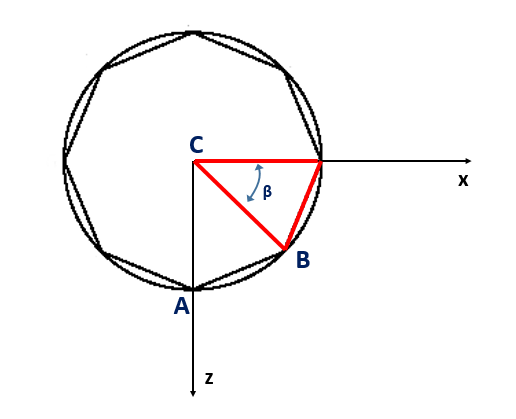
\includegraphics[scale=0.5]{imagens/p3_circulo.png}
	\caption{Esquema representativo do círculo}
	\label{p1:fig:p3_circulo}
\end{figure}

Para se saber os pontos de um círculo foram usadas coordenadas polares. Para tal a classe \textit{CoordsPolares} foi usada (ver secção \ref{p1:coordsPolares}).

O número de triângulos de um círculo corresponde ao número de ``fatias'' que se pretende e com isso é possível calcular a variação do angulo $\theta$ em cada iteração para se obter os pontos.

Tal como o plano, um círculo também tem uma orientação. Caso se pretenda desenhar o círculo virado no sentido positivo do eixo dos Y, a ordem de colocação dos pontos deverá ser C-A-B. Caso se pretenda desenhar o círculo virado no sentido negativo do eixo dos Y, a ordem de colocação dos pontos deverá ser C-B-A.

A função responsável pelo desenho de círculos é a função \textit{criaCirculo()}, cujo pseudo-código é o seguinte:

\begin{Verbatim}
Figura& criaCirculo(Ponto3D C, float raio, int fatias, 
int orientacao) {

CoordsPolares A, B;
float dAz = (2.0 * M_PI) / (fatias + 0.0f);

if (orientacao == 1) {
for (int i = 0; i < fatias; i++) {
A = CoordsPolares(C, raio, dAz*i);
B = CoordsPolares(C, raio, dAz*(i + 1));

Gera pontos pela ordem C-A-B
}
}
else {
for (int i = 0; i < fatias; i++) {
A = CoordsPolares(C, raio, dAz*i);
B = CoordsPolares(C, raio, dAz*(i + 1));

Gera pontos pela ordem C-A-B
}
}


return *this;
}



\end{Verbatim}

\newpage
\subsection{Gerar Cone}

Para gerar um cone, o utilizador deve efetuar o comando com a seguinte sintaxe:

\begin{Verbatim}
Gerador cone raio altura fatias camadas ficheiro
\end{Verbatim}

A base do cone corresponde a um círculo virado no sentido negativo dom eixo dos Y. Como apresentado na secção \ref{p3:circulo}, a função \textit{criaCirculo()} permite fazer isto. Resta apenas gerar os pontos para a superfície ``curva'' do cone. Para essa superfício, abordagem seguida foi a de fazer o cone camada a camada. As fatias partem cada camada numa espécie ``rectângulos'' como o que se mostra na figura \ref{p1:fig:p3_seccaoCone_edit}.


\begin{figure}[<+htpb+>]
	\centering
	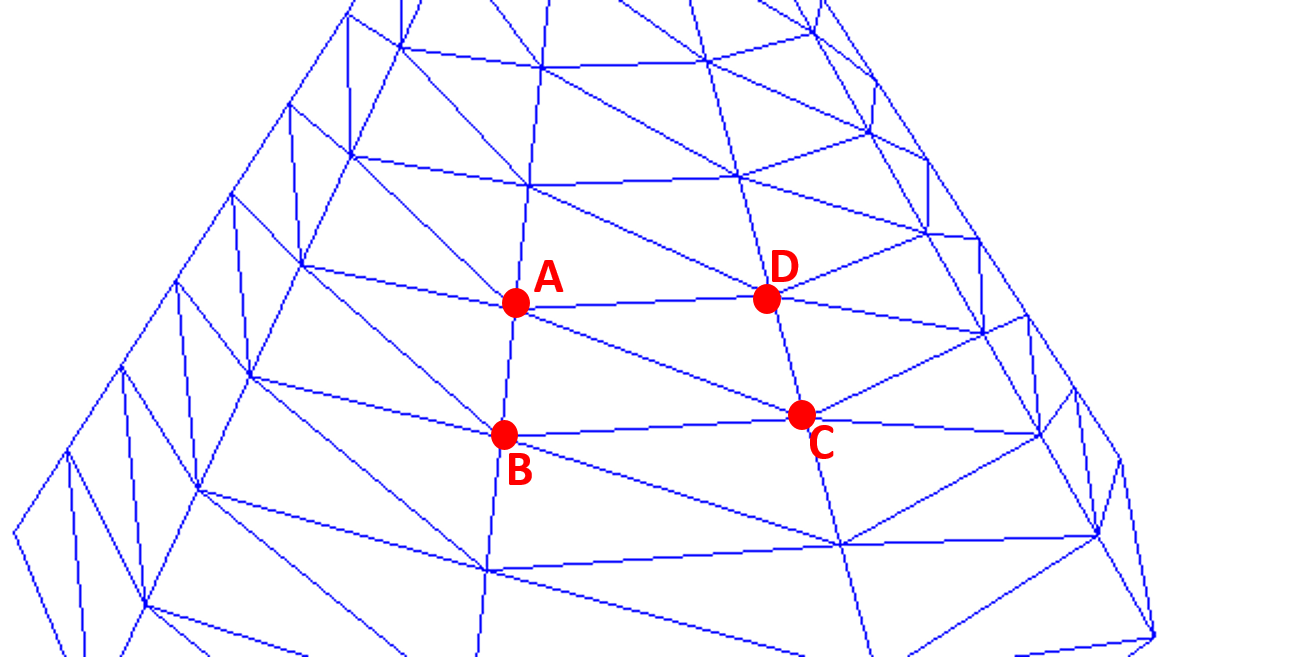
\includegraphics[scale=0.5]{imagens/p3_seccaoCone_edit.png}
	\caption{Esquema representativo de uma fatia de uma camada do cone (Pontos A,B,C e D)}
	\label{p1:fig:p3_seccaoCone_edit}
\end{figure}

Ou seja, é possível construir uma fatia de uma dada camada com os pontos A,B,C e D. É no entanto necessário saber as coordenadas destes pontos. Para tal, foram usadas coordenadas polares, com auxílio mais uma vez da classe \textit{CoordsPolares}. Podemos ver os pontos A e D como pertencentes a um mesmo círculo, com centro no centro do cone. Da mesma forma, também os pontos B e C se encontram num mesmo círculo, com raio maior do que o círculo onde estão os pontos A e D. O raio dos dois círculos em que estes dois conjuntos de pontos se encontram difere, no entanto é fácil perceber que o raio do círculo depende da camada que se está a considerar. Por exemplo, se virmos a base do cone como um círculo de raio $r$, então o círculo correspondente à camada de cima terá raio $r - (r/camadas)$. A figura \ref{p1:fig:p3_conePerfil} pretende ilustrar tal situação para um exemplo de 3 camadas.

\begin{figure}[<+htpb+>]
	\centering
	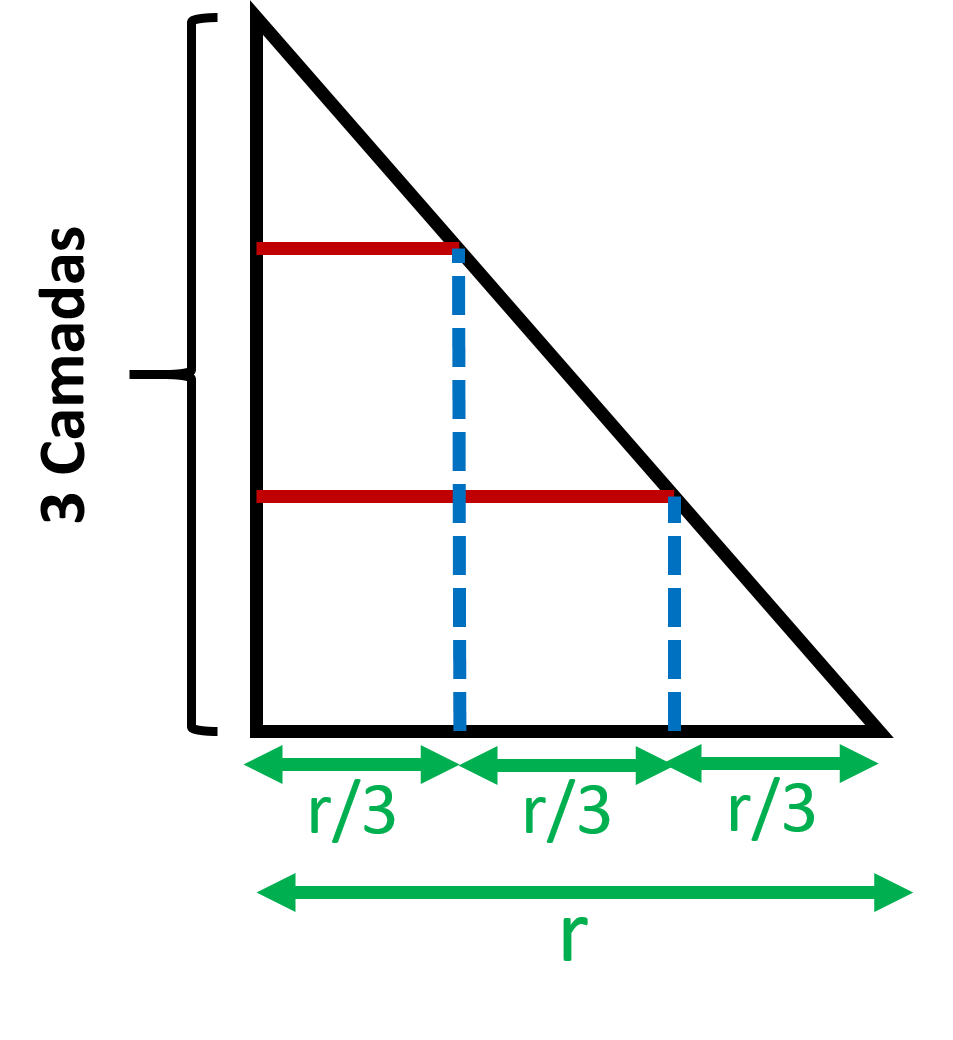
\includegraphics[scale=0.5]{imagens/p3_conePerfil.png}
	\caption{O círculo da camada superior à que se considera tem sempre raio $r - (r/camadas)$}
	\label{p1:fig:p3_conePerfil}
\end{figure}

Saber o centro de cada um dos círculos do cone também é simples. Os centros dos círculos encontram-se todos no centro do cone, a única coisa que varia em cada um é a coordenada Y cuja diferença para a coordenada Y da camada anterior é $altura / camadas$.

Visto que a classe de \textit{CoordsPolares} é capaz de dar coordenadas cartesianas sendo indicado um centro, um raio e um ângulo e tendo em conta o exposto anteriormente então a função criaCone() fica simplesmente:

\begin{Verbatim}
Figura& criaCone(Ponto3D centroCone, float altura, 
float raio, int camadas, int fatias) {

float dRaio = raio / (camadas + 0.0f);
float dAltura = altura / (camadas + 0.0f);
float dAz = (2.0 * M_PI) / (fatias + 0.0f);
float meiaAltura = altura / 2.0f;

Calcula coordendadas do centro da base

Cria circulo no centro da base virado no sentido
negativo do eixo dos Y.

for (int i = 0; i < camadas; i++) {
for (int j = 0; j < fatias; j++) {
Calcula o centro do circulo "de baixo" da
camada que se está a considerar

Calcula o centro do circulo "de cima" da
camada que se está a considerar

A = CoordsPolares(cCima,
raio - (dRaio*(i + 1.0)),
dAz * j);
B = CoordsPolares(cBaixo,
raio - (dRaio*(i + 0.0)),
dAz * j);
C = CoordsPolares(cBaixo,
raio - (dRaio*(i + 0.0)),
dAz * (j + 1.0));
D = CoordsPolares(cCima,
raio - (dRaio*(i + 1.0)),
dAz * (j + 1.0));

Gera os pontos pela ordem A-B-C-C-D-A
}
}

return *this;
}
\end{Verbatim}

\begin{figure}[<+htpb+>]
	\centering
	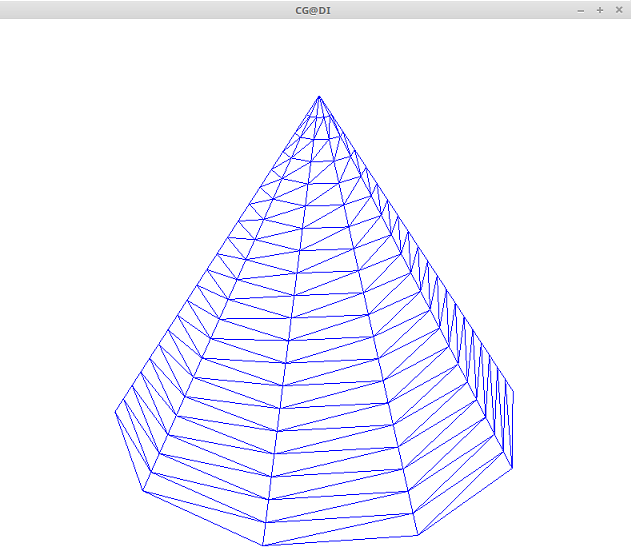
\includegraphics[scale=0.5]{imagens/p3_cone_2_3_10_10.png}
	\caption{Exemplo de cone gerado, com 2 de raio de base, 3 de altura, 10 camadas e 10 fatias}
	\label{p1:fig:p3_cone_2_3_10_10}
\end{figure}

\newpage
\subsection{Gerar Esfera}

Para gerar uma esfera, o utilizador deve efetuar o comando com a seguinte sintaxe:

\begin{Verbatim}
Gerador sphere raio fatias camadas ficheiro
\end{Verbatim}

Os pontos da esfera foram gerados à custa de coordenadas esféricas, nomeadamente com o auxílio da classe \textit{CoordsEsfericas}.

À semehança do cone também para a esfera é possível gerar uma fatia de uma determinada camada usando 4 pontos conforme mostrado na figura \ref{p1:fig:p3_esferaSeccao_edit}.

\begin{figure}[<+htpb+>]
	\centering
	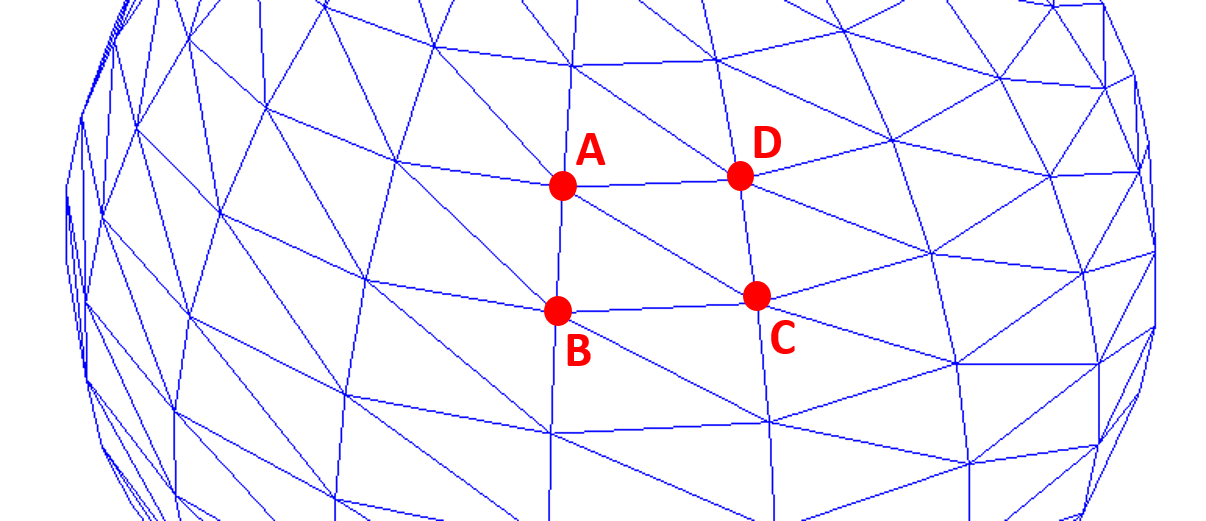
\includegraphics[scale=0.5]{imagens/p3_esferaSeccao_edit.png}
	\caption{Esquema representativo de uma fatia de uma camada da esfera (Pontos A,B,C e D)}
	\label{p1:fig:p3_esferaSeccao_edit}
\end{figure}

Também para a esfera a abordagem seguida foi a de construir camada a camada, começando pela camada de cima. A determinação das coordenadas dos pontos A, B, C e D é simples. Uma vez que se está a usar a classe \textit{CoordsEsfericas}, a única coisa que se tem que perceber para usar a classe é de que forma variam os ângulos polar e azimuth entre camadas e fatias. Ora, tendo $c$ camadas, sabe-se que a diferença em termos de ângulo polar de um ponto que esteja numa camada superior para outro que esteja numa camada imediatamente inferior é de $\pi / c$. Por outro lado, se considerarmos $f$ fatias, a diferença do ângulo azimuth de um ponto para outro que esteja numa fatia imediatamente a seguir é de $(2 \times \pi) / f$. Assim temos o seguinte pseudo-código:

\begin{Verbatim}
Figura& criaEsfera(int fatias, int camadas, float raio) {

float deltaPolar = M_PI / (camadas+0.0f);
float deltaAz = (2.0 * M_PI) / (fatias+0.0f);

for (int i = 0; i < camadas; i++) {
for (int j = 0; j < fatias; j++) {
A = CoordsEsfericas(raio, 
deltaAz * (j + 0.0f), 
deltaPolar * (i+0.0f));
B = CoordsEsfericas(raio,
deltaAz * (j + 0.0f), 
deltaPolar * (i+1.0f));
C = CoordsEsfericas(raio,
deltaAz * (j + 1.0f),
deltaPolar * (i+1.0f));
D = CoordsEsfericas(raio,
deltaAz * (j + 1.0f),
deltaPolar * (i+0.0f));

Gera pontos pela ordem A-B-C-C-D-A

}
}

return *this;
}
\end{Verbatim}

\begin{figure}[<+htpb+>]
	\centering
	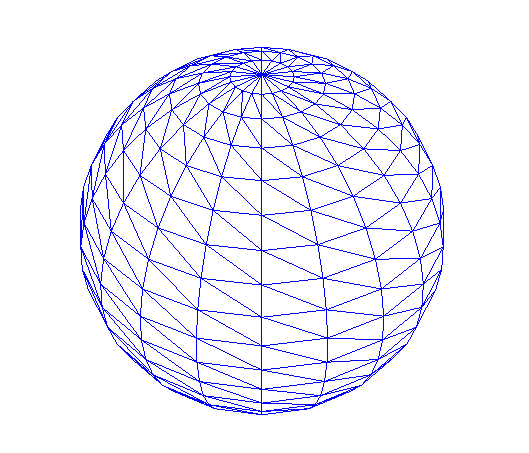
\includegraphics[scale=0.5]{imagens/p3_esfera_2_20_20.png}
	\caption{Exemplo de esfera gerada, com 2 de raio, 20 camadas e 20 fatias}
	\label{p1:fig:p3_esfera_2_20_20}
\end{figure}




\chapter{Gerador1}
\label{cap:p1}

Nesta secção apresentam-se as classes usadas. Tanto o motor como o gerador recorrem extensivamente a estas classes para desempenhar as suas funções. Algumas destas classes são recorrentes e usadas mais que uma vez em diferentes contextos. Assim, antes de introduzir como funciona o motor e o gerador é importante primeiro perceber quais são as classes que ambos usam, bem como a função de cada uma.

O objectivo de construção destas classes foi simplificar a construção do motor e gerador apenas. Nesta primeira etapa, foram deixadas para segundo plano questões como a modularidade e encapsulamento de dados, embora seja algo a considerar em etapas posteriores do trabalho.

\section{Ponto3D}

Tanto o gerador como o motor trabalham com pontos. Assim, foi criada uma classe que representa o conceito de um ponto num espaço 3D:

\begin{Verbatim}
	struct Ponto3D {
		float x, y, z;
	};
\end{Verbatim}

Como se pode verificar, esta classe é bastante simples e apenas contém 3 variáveis do tipo \textit{float}, correspondentes às coordenadas cartesianas de um ponto num espaço 3D.

Visto nenhuma das aplicações exigir operações complexas sobre pontos, esta classe foi mantida simples. De facto, tanto motor como gerador, apenas precisam de ler valores de coordenadas de pontos e ocasionalmente mudar os seus valores, o que pode ser feito directamente acedendo às variáveis desta classe.

O facto desta classe ser simples e não ter nenhuma função ou construtor faz com que seja considerada pelo C++ como uma \textit{aggregate class}. Este tipo de classe tem propriedades específicas, nomeadamente uma inicialização fácil e intuitiva das instâncias, o que contribui também para código mais fácil de ler. Esse fator foi fundamental para a decisão de manter a classe simples.

\newpage
\section{CoordsPolares}
\label{p1:coordsPolares}
Esta classe pretende abstrair os cálculos relacionados com coordenadas polares. A ideia é poderem ser criadas instâncias desta classe indicando os parâmetros correspondentes a coordenadas polares e as correspondentes coordenadas cartesianas poderem ser obtidas facilmente a partir da instância.

As coordenadas polares são constituídas por um ponto central, um raio e por um ângulo $\alpha$ (também designado por ângulo azimuth) e permitem localizar um ponto num plano conforme se ilustra na figura \ref{p1:fig:p1_polarCoords}:

\begin{figure}[<+htpb+>]
	\centering
	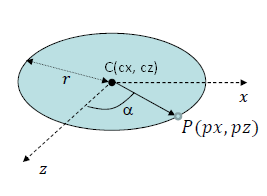
\includegraphics[scale=1.0]{imagens/p1_polarCoords.png}
	\caption{Localização de um ponto P(px,py,pz) segundo um centro C(cx,cy,cz), um ângulo azimuth ($\alpha$) e um raio $r$}
	\label{p1:fig:p1_polarCoords}
\end{figure}

Designando o ponto central como C(cx,cy,cz) e um ponto P(px,py,pz) que se pretende localizar, temos que as coordenadas px e py podem ser obtidas da seguinte forma:\\

	$px = cx + r \times sin(\alpha)$
	
	$py = cy$
	
	$pz = cz + r \times cos(\alpha)$\\

A classe \textit{CoordsPolares} representa apenas uma forma fácil de trabalhar com este sistema de coordenadas. Esta classe possui variáveis de instância relacionadas com as suas coordenadas polares e cartesianas:

\begin{Verbatim}
	//Centro a partir do qual se 
	//considera as coordenadas polares
	Ponto3D centro;
	//Coordenadas polares
	float raio, azimuth;
	//Coordenadas rectangulares correspondentes 
	//às coordenadas polares
	Ponto3D cCartesianas;
\end{Verbatim}

O ponto chave desta classe é que as variáveis das coordenadas polares e cartesianas referem-se sempre ao mesmo ponto. Sempre que um dos parâmetros é alterado (através de uma das funções disponibilizadas), todos os restantes são actualizados em conformidade.

A classe tem um único construtor:

\begin{Verbatim}
CoordsPolares(Ponto3D c, float r, float az);
\end{Verbatim}

Neste construtor são pedidos os parâmetros referentes às coordenadas polares. O primeiro parâmetro \textit{c} corresponde ao ponto central, o segundo parâmetro r corresponde ao raio e o último parâmetro corresponde ao ângulo azimuth ($\alpha$). Ao receber estas coordenadas polares, o construtor seguidamente atualiza as variáveis de instância em conformidade, nomeadamente coloca na variável de instância \textit{cCartesianas} as coordenadas cartesianas correspondentes às coordenadas polares passadas como argumento. Essa actualização é feita pela função \textit{refreshCartesianas()}:

\begin{Verbatim}
void refreshCartesianas(){
	cRectangulares.x = centro.x + raio * sin(azimuth);
	cRectangulares.y = centro.y;
	cRectangulares.z = centro.z + raio * cos(azimuth);
}
\end{Verbatim}

Como se pode ver, esta função implementa apenas as fórmulas apresentadas anteriormente. Esta função é privada à classe, por isso não pode ser chamada em qualquer parte do código. É a própria classe que se responsabiliza por chamar esta função sempre que necessário.

Assim, dada uma instância desta classe é sempre possível saber as coordenadas cartesianas correspondentes através da função \textit{toCartesianas()}:

\begin{Verbatim}
Ponto3D toCartesianas() {
	return cCartesianas;
}
\end{Verbatim}


\section{CoordsEsfericas}
\label{p1:cEsfericas}
Esta classe pretende abstrair os cálculos relacionados com coordenadas esféricas. A ideia é poderem ser criadas instâncias desta classe indicando os parâmetros correspondentes a coordenadas esféricas e as correspondentes coordenadas cartesianas poderem ser obtidas facilmente a partir da instância. É também possível fazer o inverso, ou seja, indicar um ponto com coordenadas cartesianas e obter as respectivas coordenadas esféricas.

As coordenadas esféricas são constituídas por um raio $r$, por um ângulo $\theta$ (também designado por ângulo azimuth) e um ângulo $\phi$ (também designado por ângulo polar), conforme apresentado na figura \ref{p1:fig:p1_sphericalCoords}:

\begin{figure}[<+htpb+>]
	\centering
	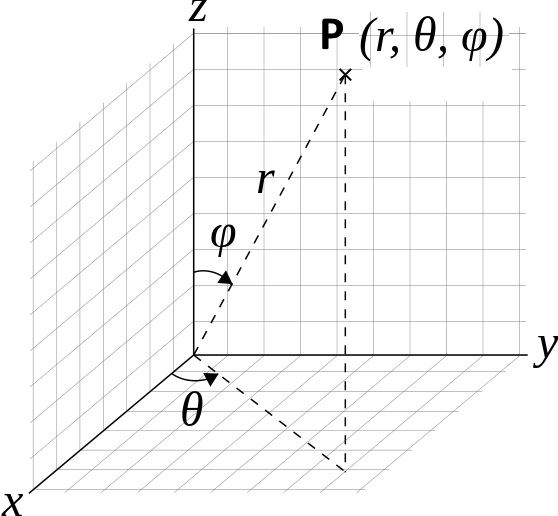
\includegraphics[scale=0.5]{imagens/p1_sphericalCoords.png}
	\caption{Localização de um ponto P segundo coordenadas esféricas}
	\label{p1:fig:p1_sphericalCoords}
\end{figure}

É possível saber as coordenadas cartesianas de um ponto P(px,py,pz) a partir das suas coordenadas esféricas através das seguintes fórmulas:\\

		$px = r \times cos(\theta) \times sin(\phi)$
		
		$py = r \times sin(\theta) \times sin(\phi) $
		
		$pz = r \times cos(\phi)$\\


Por outro lado, consegue-se saber também as coordenas esféricas de um ponto a partir das suas coordenadas cartesianas de acordo com as seguintes fórmulas:\\

		$r = \sqrt{px^2 + py^2 + pz^2}$
		
		$\theta = \arctan(py \backslash px) $
		
		$\phi = \arccos (pz \backslash r)$\\

De referir que ao contrário da classe \textit{CoordsPolares}, nesta classe optou-se por não se considerar um centro. Assume-se o centro como sendo (0.0,0.0,0.0) sempre. Considerou-se esta simplificação razoável na medida em que responde aos requisitos do motor e gerador nesta primeira fase.

A classe \textit{CoordsEsfericas} tem as seguintes variáveis de instância:

\begin{Verbatim}
// Coordenadas Esfericas
float raio, azimuth_ang, polar_ang;
// Coordenadas cartesianas
Ponto3D cCartesianas;
\end{Verbatim}

O ponto chave desta classe é que as variáveis das coordenadas esféricas e cartesianas referem-se sempre ao mesmo ponto. Sempre que um dos parâmetros é alterado (através de uma das funções disponibilizadas), todos os restantes são atualizados em conformidade.

Uma instância da classe \textit{CoordsEsfericas} pode ser criada indicando os parâmetros das coordenadas esféricas (para se saber as suas coordenadas cartesianas), ou indicando um ponto em coordenadas cartesianas (do qual se pretende saber as coordenadas esféricas), através dos seguintes construtores:

\begin{Verbatim}
CoordsEsfericas(float r, float az, float polar);
CoordsEsfericas(Ponto3D pto);
\end{Verbatim}

Caso a instância seja criada a partir de coordenadas polares, o construtor calcula as coordenadas cartesianas correspondentes através da função \textit{refreshCartesianas()}:

\begin{Verbatim}
void refreshCartesianas() {
	cCartesianas.z = raio * sin(polar_ang) * cos(azimuth_ang);
	cCartesianas.x = raio * sin(polar_ang) * sin(azimuth_ang);
	cCartesianas.y = raio * cos(polar_ang);
}
\end{Verbatim}

Caso a instância seja criada a partir de coordenadas cartesianas, o construtor calcula as coordenadas polares correspondentes através da função \textit{refreshEsfericas()}:

\begin{Verbatim}
void refreshEsfericas() {
	raio = sqrt(pow(cCartesianas.x, 2) + 
		pow(cCartesianas.y, 2) + 
		pow(cCartesianas.z, 2));
	polar_ang = acos(cCartesianas.y / raio);
	azimuth_ang = atan2(cCartesianas.x, cCartesianas.z);
}
\end{Verbatim}

Estas duas funções correspondem à implementação das fórmulas apresentadas anteriormente e garantem que as variáveis de instância correspondentes às coordenadas esféricas e cartesianas se referem sempre ao mesmo ponto. Ambas são funções privadas, pelo que é a própria classe que tem a responsabilidade de as chamar sempre que é necessário atualizar valores.

A qualquer momento, é possível saber as coordenadas cartesianas de uma instância pela função \textit{toCartesianas()}

\begin{Verbatim}
Ponto3D toCartesianas() {
	return cCartesianas;
}
\end{Verbatim}

Além destas funções, a classe possui ainda funções adicionais que permitem mudar a posição do ponto representado por cada instância. Sempre que uma destas funções é chamada tanto as variáveis de instância das coordenadas polares e cartesianas são atualizadas quer pela função refreshEsfericas() ou refreshCartesianas(). Estas funções que permitem mudar a localização do ponto, garantem ainda que $0 \leq \phi \leq \pi$ e que $0 \leq \theta \leq 2 \times \pi$

\newpage

\section{Figura}

Esta classe representa uma figura que será desenhada pelo motor. Representa por isso apenas um conjunto de pontos numa determinada ordem que correspondem a triângulos, que por sua vez formam uma figura.

Por representar um conjunto de pontos, sem surpresa, a sua única variável de instância é um vector de pontos:

\begin{Verbatim}
std::vector<Ponto3D> pontos;
\end{Verbatim}

A utilidade desta classe revela-se pelas funções que disponibiliza. Em primeiro lugar, disponibiliza um conjunto de funções que quando chamadas colocam no vector \textit{pontos} os pontos necessários para o desenho de uma figura em concreto. Dessa forma, estas funções permitem criar planos, caixas, círculos, cilindros e esferas. Estas funções serão explicadas em mais detalhe quando for apresentado o gerador onde será mostrado de que forma estas funções podem ser chamadas bem como de que forma geram os pontos.

Além das funções que permitem criar figuras destaca-se ainda a função \textit{toFicheiro()}, que permite guardar os pontos da figura num ficheiro cujo nome é passado como argumento.

\begin{Verbatim}
void toFicheiro(std::string filePath)
\end{Verbatim}

É ainda possível obter os pontos da figura pela função \textit{getPontos()}:

\begin{Verbatim}
std::vector<Ponto3D> getPontos()
\end{Verbatim}

\section{TinyXML-2}

Esta biblioteca foi usada para auxílio à leitura de ficheiros XML por parte do motor e pode ser encontrada no endereço: http://www.grinninglizard.com/tinyxml2/
